\section{Make a new Hexagonal Core}

First, we'll need to create a new hexagonal core.

\begin{figure}[H]
	\begin{center}
		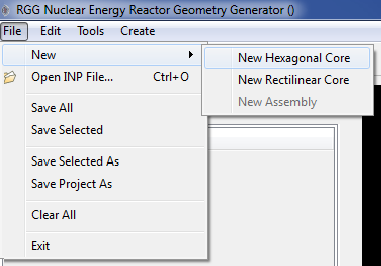
\includegraphics[width=0.5\linewidth]{Images/hex-1.png}
		\caption{Select the option to create a new hexagonal core.}
		\label{fig:Hex1}
	\end{center}
\end{figure}

The two panels on the left of the application will change.  We'll now see that the inputs panel contains an item named ``Core" with a subitem ``Assy1."  The core panel should show a hexagon labeled ``Assy1." Confirm that your application looks similar to what's shown in ~\ref{fig:Hex2}.

\begin{figure}[H]
	\begin{center}
		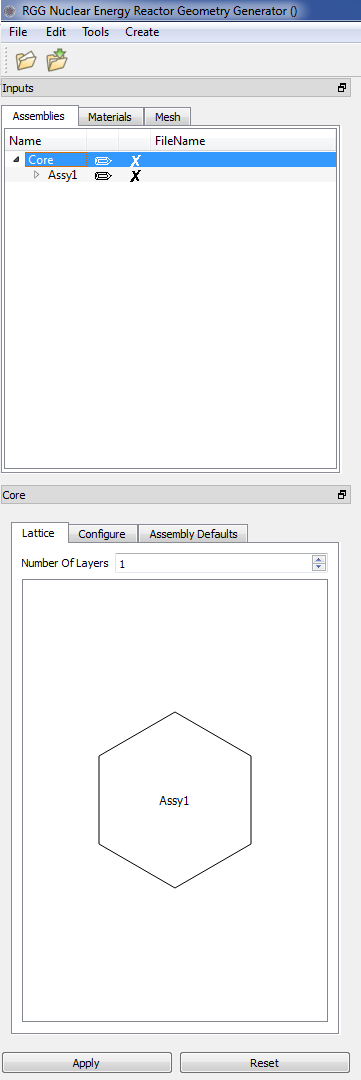
\includegraphics[width=0.2\linewidth]{Images/hex-2.png}
		\caption{The inputs and core panels after creating a new hexagonal core.}
		\label{fig:Hex2}
	\end{center}
\end{figure}

Next, we'll specify how many layers we'd like our lattice to have.  In the core panel, either type in the number of desired layers or use the buttons to the right of the field to increment and decrement the number.  The panel should look something like what's displayed in ~\ref{fig:Hex3}.

\begin{figure}[H]
	\begin{center}
		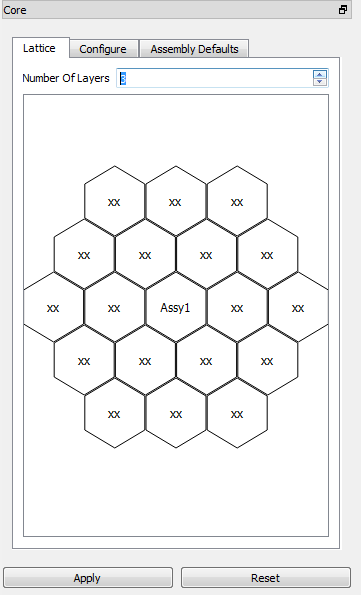
\includegraphics[width=0.5\linewidth]{Images/hex-3.png}
		\caption{Updating the number of layers of the core.}
		\label{fig:Hex3}
	\end{center}
\end{figure}

Be sure to click the apply button below to see apply changes.

\begin{figure}[H]
	\begin{center}
		
\includegraphics[width=0.5\linewidth]{Images/hex-4.png}
		\caption{The apply button.}
		\label{fig:Hex4}
	\end{center}
\end{figure}

\section{Configuring the Assembly}
We need to configure the hexagonal ducts and pins we'll create to be rotated by 30 degrees to avoid interference from the different cells.  To do this, first ensure that you're clicking on the assembly we created, as shown in ~\ref{fig:Hex15}.

\begin{figure}[H]
	\begin{center}
		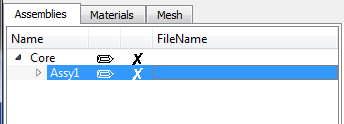
\includegraphics[width=0.5\linewidth]{Images/hex-15.png}
		\caption{Clicking on our assembly.}
		\label{fig:Hex15}
	\end{center}
\end{figure}

Then, we need to click on the configure tab in the lower panel, and scroll down to the section labeled transform.  Click the Add Rotation button.

\begin{figure}[H]
	\begin{center}
		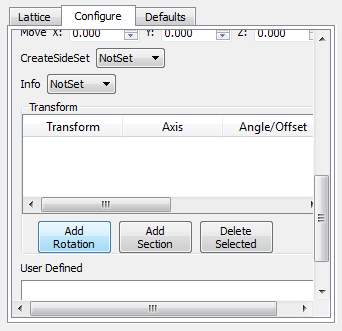
\includegraphics[width=0.5\linewidth]{Images/hex-16.png}
		\caption{Assembly transformations.}
		\label{fig:Hex16}
	\end{center}
\end{figure}

We need to change this rotation to be 30 degrees.  Enter 30 as shown in ~\ref{fig:Hex17}.

\begin{figure}[H]
	\begin{center}
		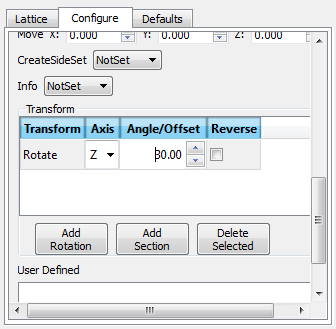
\includegraphics[width=0.5\linewidth]{Images/hex-17.png}
		\caption{Adding the 30 degree transformation.}
		\label{fig:Hex17}
	\end{center}
\end{figure}

As always, please click Apply to make sure that your changes are saved.

\section{Adding a duct to the Assembly}

\subsection{Creating the Duct}

Now that we have set up our core and configured the assembly, we need to create a duct.  To do this, follow ~\ref{fig:Hex5}.

\begin{figure}[H]
	\begin{center}
		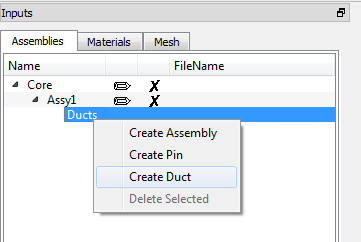
\includegraphics[width=0.5\linewidth]{Images/hex-5.png}
		\caption{Creating a duct.}
		\label{fig:Hex5}
	\end{center}
\end{figure}

Your screen should now look like this:

\begin{figure}[H]
	\begin{center}
		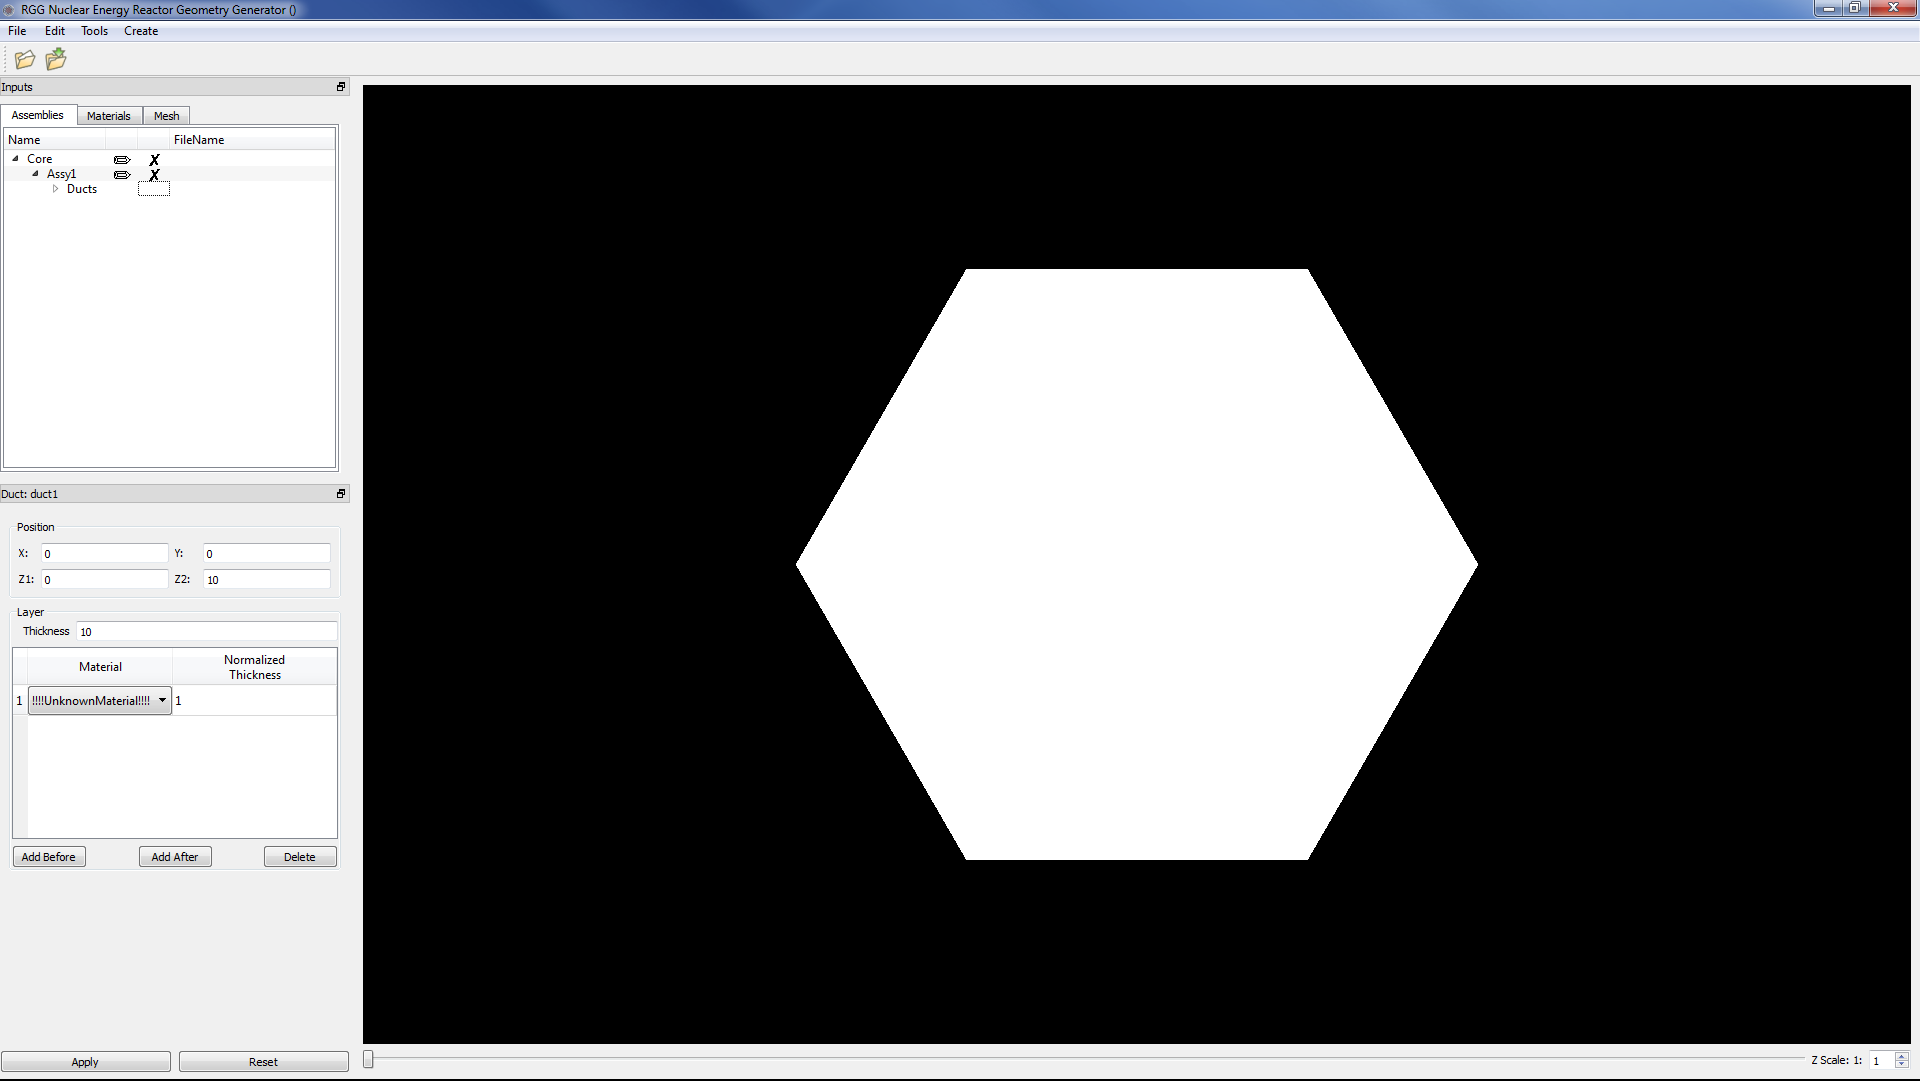
\includegraphics[width=0.85\linewidth]{Images/hex-6.png}
		\caption{Your screen after adding duct.}
		\label{fig:Hex6}
	\end{center}
\end{figure}

\subsection{Configuring Duct}

We now need to configure the duct we created.  In the inputs panel, select the duct.  This will change the lower panel to show the materials of the duct and the normalized radii of those materials.  For this duct, we'll stay simple and make the material water.  Change the material type to water by clicking the drop-down and selecting ``water."

\begin{figure}[H]
	\begin{center}
		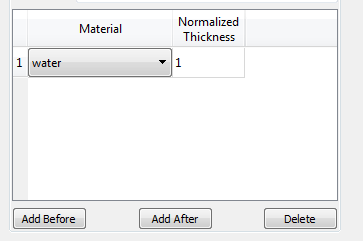
\includegraphics[width=0.5\linewidth]{Images/hex-7.png}
		\caption{Selecting water as our material.}
		\label{fig:Hex7}
	\end{center}
\end{figure}

Your screen should now look like ~\ref{fig:Hex8}.

\begin{figure}[H]
	\begin{center}
		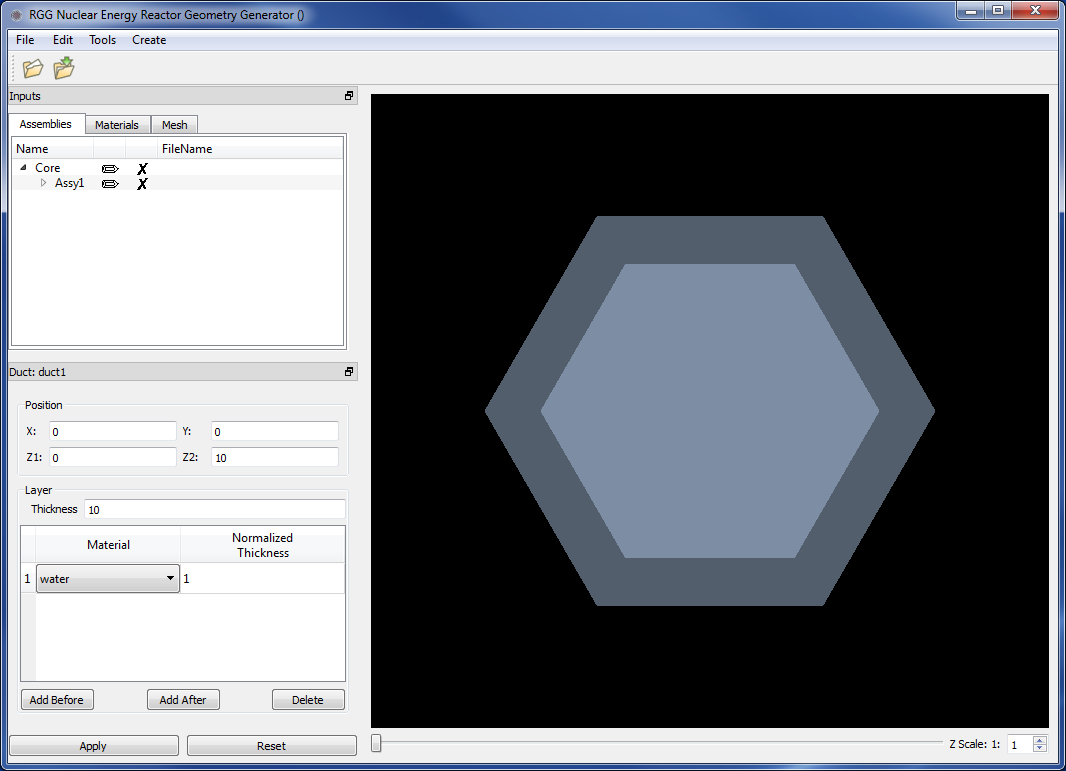
\includegraphics[width=0.5\linewidth]{Images/hex-8.png}
		\caption{Creating a duct.}
		\label{fig:Hex8}
	\end{center}
\end{figure}

\section{Adding a Pin}
\subsection{Creating a Pin}

To create a pin in the assembly, right click on the name of the assembly and select ``Create Pin."

\begin{figure}[H]
	\begin{center}
		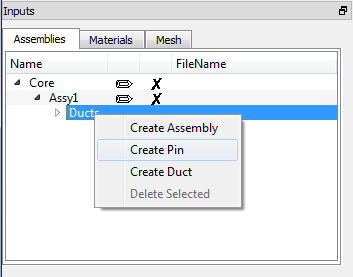
\includegraphics[width=0.5\linewidth]{Images/hex-9.png}
		\caption{Creating a pin.}
		\label{fig:Hex9}
	\end{center}
\end{figure}

\subsection{Configuring the Pin}

You can edit the name, label, pitch, and cell material of the pin.  Refer to ~\ref{fig:Hex10} to see how to change them.  We will leave them to the defaults.

\begin{figure}[H]
	\begin{center}
		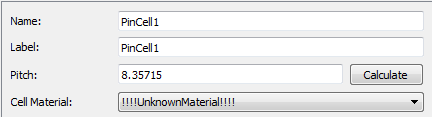
\includegraphics[width=0.5\linewidth]{Images/hex-10.png}
		\caption{Name, label, pitch, and cell material for a pin.}
		\label{fig:Hex10}
	\end{center}
\end{figure}

We now need to add pieces of the pin.  There are two kinds of pin pieces: frustrums and cylinders.  We'll add a cylinder by clicking the add button.

\begin{figure}[H]
	\begin{center}
		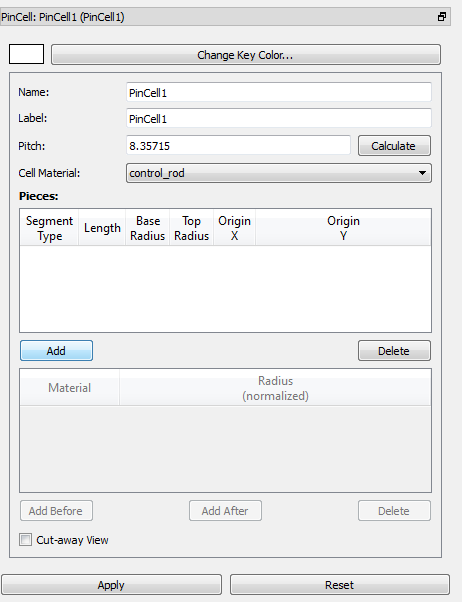
\includegraphics[width=0.5\linewidth]{Images/hex-11.png}
		\caption{Adding a pin piece.}
		\label{fig:Hex11}
	\end{center}
\end{figure}

Then, confirm that our segment type is a cylinder, and that the sum of the length of the segments is equal to the length of the duct (10).

\begin{figure}[H]
	\begin{center}
		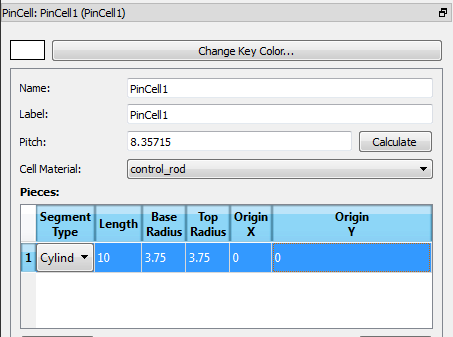
\includegraphics[width=0.5\linewidth]{Images/hex-12.png}
		\caption{Confirming our cylinder's configuration.}
		\label{fig:Hex12}
	\end{center}
\end{figure}

Now, we're going to modify the material of this cylinder.  We'll make this a control rod, so we'll change the material to match.

\begin{figure}[H]
	\begin{center}
		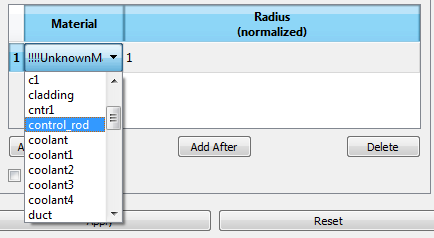
\includegraphics[width=0.5\linewidth]{Images/hex-13.png}
		\caption{Changing the material to be a control rod.}
		\label{fig:Hex13}
	\end{center}
\end{figure}

Be sure to press apply to ensure your changes go into effect.

We should see a screen like the after we're done:

\begin{figure}[H]
	\begin{center}
		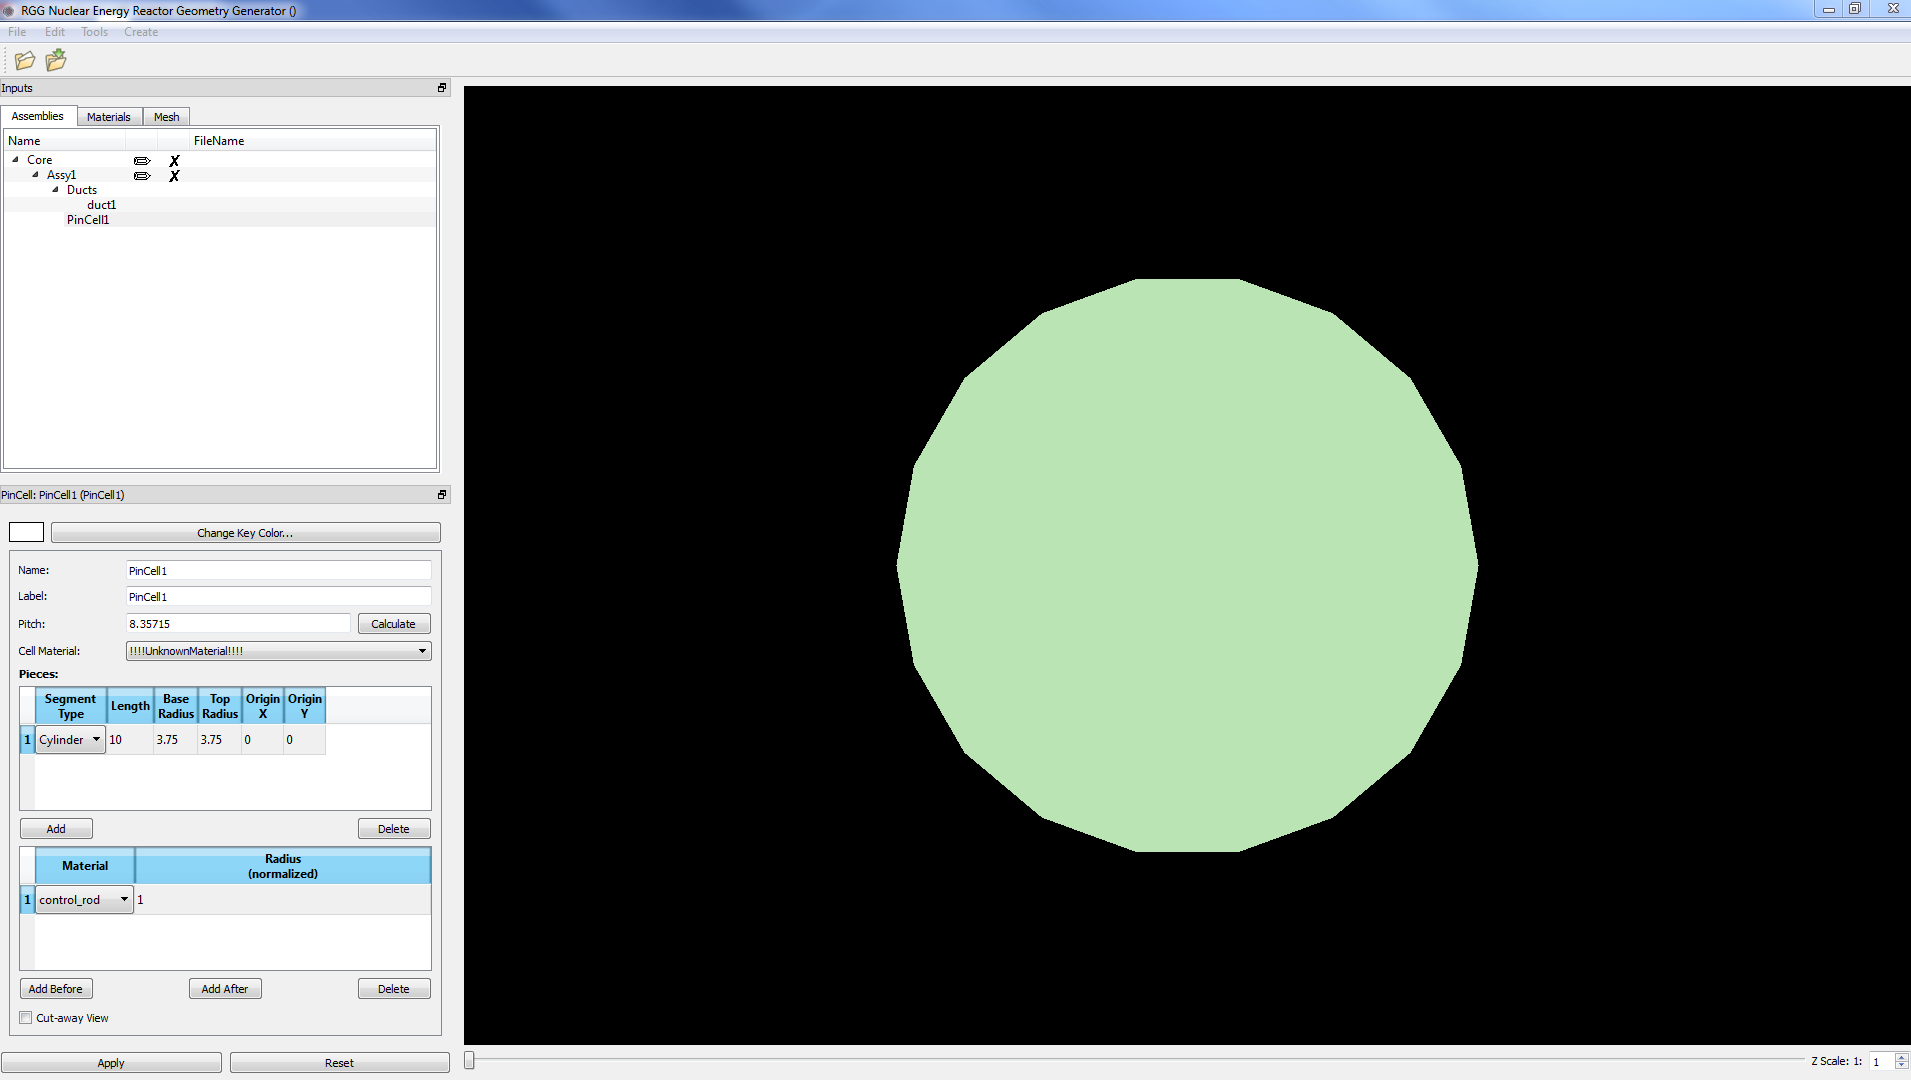
\includegraphics[width=0.85\linewidth]{Images/hex-14.png}
		\caption{After adding the cylinder.}
		\label{fig:Hex14}
	\end{center}
\end{figure}

Next, we need to add this pin to our assembly lattice.  Make sure you select ``Assy1" in the inputs menu.  Click the lattice tab in the lower panel, and right click on the hexagon to bring up a list of available pins.  Select our pin.

\begin{figure}[H]
	\begin{center}
		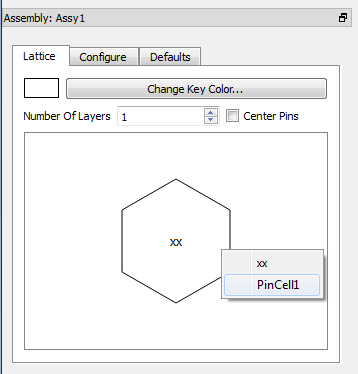
\includegraphics[width=0.5\linewidth]{Images/hex-18.png}
		\caption{Selecting our pin for the assembly.}
		\label{fig:Hex18}
	\end{center}
\end{figure}

Click the apply button to save your changes.

\section{Populating core with our assembly}

Click on our assembly (``Assy1") in the inputs pane.  In the lower pane, click on the lattice tab.  To add the assembly to any of the cells, right click to bring up a list of available assemblies, and then click on the assembly you'd like.

\begin{figure}[H]
	\begin{center}
		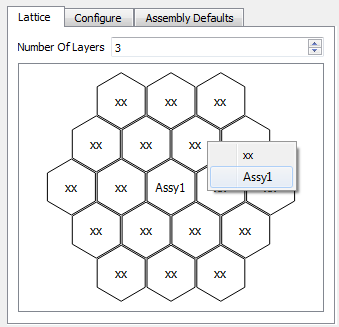
\includegraphics[width=0.5\linewidth]{Images/hex-19.png}
		\caption{Selecting assembly for a cell.}
		\label{fig:Hex19}
	\end{center}
\end{figure}

We'll select Assy1 because that's the name of the assembly we'd like.  Make sure to click the apply button to make sure that the changes we've made are applied.  Your screen should look like the following when you're done.

\begin{figure}[H]
	\begin{center}
		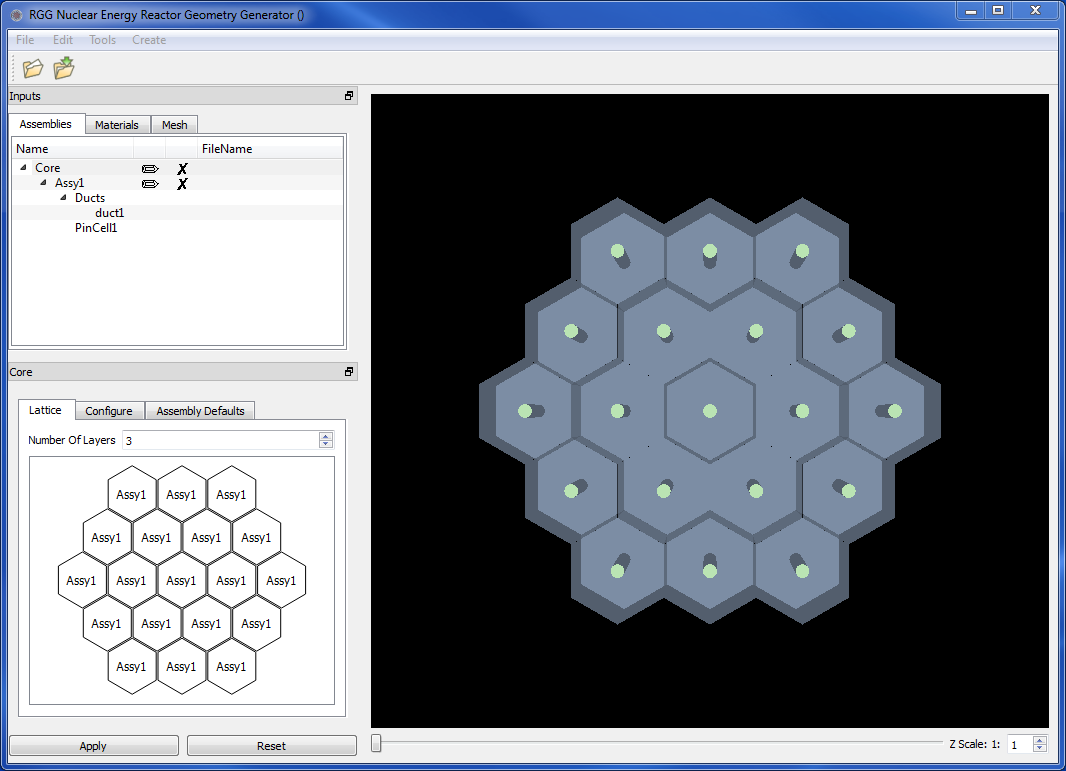
\includegraphics[width=0.85\linewidth]{Images/hex-20.png}
		\caption{Final view.}
		\label{fig:Hex20}
	\end{center}
\end{figure}

Congratulations!  You've made a hexagonal core!